\documentclass[10pt,letterpaper]{article}
\usepackage[utf8]{inputenc}
\usepackage[T1]{fontenc}
\usepackage[margin=0.6in]{geometry}
\usepackage{amsmath,amssymb,mathtools,graphicx,booktabs,xcolor,hyperref}
\setlength{\parindent}{0pt}
\setlength{\parskip}{5pt}
\begin{document}

\section*{Block S5 Solutions: Series AC RLC Concepts, Inductance, Reactance \& Capacitance}

  \textbf{Companion Key to:} \texttt{Block\_S5\_Exercises\_AC\_RLC\_Reactance.pdf} ~|~
  \textbf{Verification:} Cross-checked via Spec v2 AC Phasor Solver


\subsection*{01 $\cdot$ Solutions: Reactance Proofs \& Solenoid Energy Density \hfill [12 Points]}


  \subsubsection*{(a) Differential Proofs of $X_L = \omega L$ and $X_C = \frac{1}{\omega C}$ [6 points]}
  \begin{itemize}
    \item \textbf{Inductor ($v_L = L\frac{di}{dt}$) [3 pts]:} With $i(t) = I_0\cos(\omega t)$:
    $$v_L(t) = L\frac{d}{dt}[I_0\cos(\omega t)] = -\omega L I_0 \sin(\omega t) = (\omega L I_0)\cos\left(\omega t + \frac{\pi}{2}\right) = V_{L,0}\cos\left(\omega t + \frac{\pi}{2}\right).$$
    Thus $V_{L,0} = I_0 X_L$ with $X_L = \omega L$, and $v_L(t)$ \textbf{leads} $i(t)$ by $+90^\circ$ ($+\pi/2\text{ rad}$).
    \item \textbf{Capacitor ($v_C = \frac{1}{C}\int i\,dt$) [3 pts]:} Integrating $i(t) = I_0\cos(\omega t)$:
    $$v_C(t) = \frac{1}{C}\int I_0\cos(\omega t)\,dt = \frac{I_0}{\omega C}\sin(\omega t) = \left(\frac{I_0}{\omega C}\right)\cos\left(\omega t - \frac{\pi}{2}\right) = V_{C,0}\cos\left(\omega t - \frac{\pi}{2}\right).$$
    Thus $V_{C,0} = I_0 X_C$ with $X_C = \dfrac{1}{\omega C}$, and $v_C(t)$ \textbf{lags} $i(t)$ by $-90^\circ$ ($-\pi/2\text{ rad}$).
  \end{itemize}

  \subsubsection*{(b) Solenoid Self-Inductance $L = \frac{\mu_0 N^2 A}{\ell}$ \& Energy Density $u_B = \frac{B^2}{2\mu_0}$ [6 points]}
  \begin{itemize}
    \item \textbf{Inductance [3 pts]:} Applying Amp\`ere's law $\oint \mathbf{B}\cdot d\mathbf{l} = \mu_0 I_{\text{enc}}$ to a rectangle of width $w$ enclosing $\frac{N}{\ell}w$ turns gives $B w = \mu_0 \left(\frac{N}{\ell}w\right)I \implies B = \frac{\mu_0 N I}{\ell}$. Flux through one turn is $\Phi_B = BA = \frac{\mu_0 N I A}{\ell}$, so total flux linkage is $N\Phi_B = \frac{\mu_0 N^2 A}{\ell}I = LI \implies L = \dfrac{\mu_0 N^2 A}{\ell}$.
    \item \textbf{Magnetic Energy \& Density [3 pts]:} $U_B = \int_0^I L i\,di = \frac{1}{2}LI^2 = \frac{1}{2}\left(\frac{\mu_0 N^2 A}{\ell}\right)I^2$. Dividing by the volume $V_{\text{vol}} = A\ell$ and substituting $I = \frac{B\ell}{\mu_0 N}$:
    $$u_B = \frac{U_B}{A\ell} = \frac{1}{2}\mu_0 \left(\frac{N I}{\ell}\right)^2 = \frac{1}{2}\mu_0 \left(\frac{B}{\mu_0}\right)^2 = \frac{B^2}{2\mu_0}. \quad \blacksquare$$
  \end{itemize}

Final Key (Ex 01): ~ $X_L = \omega L$ ($+90^\circ$ lead), $X_C = \frac{1}{\omega C}$ ($-90^\circ$ lag) ~|~ $L = \dfrac{\mu_0 N^2 A}{\ell}$, ~ $U_B = \frac{1}{2}LI^2$, ~ $u_B = \dfrac{B^2}{2\mu_0}$

\subsection*{02 $\cdot$ Solutions: 10-Blank Conceptual Cloze \& Resonance Self-Check \hfill [10 Points]}


  \textbf{Cloze Key (1 pt each = 10 pts; 4 unused distractors):} (a) \texttt{magnetic field}; (b) \texttt{in phase with}; (c) \texttt{leads}; (d) \texttt{lags}; (e) \texttt{open circuit ($X_C \to \infty$)}; (f) \texttt{$\sqrt{R^2 + (X_L - X_C)^2}$}; (g) \texttt{$1/\sqrt{LC}$}; (h) \texttt{minimum ($Z = R$)}; (i) \texttt{capacitive ($\phi < 0$)}; (j) \texttt{$\cos\phi = R/Z$}.
  \textbf{Self-Check Explanation:} At resonance, $v_L(t) = +V_{L,0}\cos(\omega_0 t + \pi/2)$ and $v_C(t) = +V_{C,0}\cos(\omega_0 t - \pi/2) = -v_L(t)$ are $180^\circ$ out of phase at every instant, so their instantaneous sum is $v_L(t) + v_C(t) = 0$ and KVL gives $v_s(t) = v_R(t)$ even when $V_{C,0} = V_{L,0} = \frac{X_C(\omega_0)}{R}V_0 = Q V_0 > V_0$ (for Exercise 03, $Q = \frac{100\ \Omega}{50.0\ \Omega} = 2.00$, so $V_{C,0} = V_{L,0} = 240\text{ V} = 2.00\,V_0$ while $V_0 = 120\text{ V}$).



\newpage



\subsection*{03 $\cdot$ Solutions: Series AC RLC Frequency Sweep ($V_0=120\text{ V}, R=50.0\ \Omega, L=0.200\text{ H}, C=20.0\ \mu\text{F}$) \hfill [12 Points]}


  \textbf{(a) Resonance ($\omega = \omega_0$) [4 pts]:}
  $$\omega_0 = \frac{1}{\sqrt{(0.200\text{ H})(20.0\times 10^{-6}\text{ F})}} = \frac{1}{\sqrt{4.00\times 10^{-6}}} = 500\text{ rad/s}, \qquad f_0 = \frac{500}{2\pi} = 79.6\text{ Hz}.$$
  At $\omega_0 = 500\text{ rad/s}$: $X_L = (500)(0.200) = 100\ \Omega$, $X_C = \frac{1}{(500)(20.0\times 10^{-6})} = 100\ \Omega$, $Z(\omega_0) = R = 50.0\ \Omega$, $I_0 = \frac{120\text{ V}}{50.0\ \Omega} = 2.40\text{ A}$, $\phi = 0^\circ$, $P_{\text{avg}} = \frac{1}{2}(2.40)^2(50.0) = 144\text{ W}$. Peak voltages: $V_{R,0} = (2.40)(50.0) = 120\text{ V}$, $V_{L,0} = V_{C,0} = (2.40)(100) = 240\text{ V} = 2.00\,V_0$ (they cancel in anti-phase!).

  \textbf{(b) Capacitive Regime ($\omega_1 = 250\text{ rad/s} = \frac{1}{2}\omega_0$) [4 pts]:}
  $$X_L(\omega_1) = (250)(0.200) = 50.0\ \Omega, \quad X_C(\omega_1) = \frac{1}{(250)(20.0\times 10^{-6})} = 200\ \Omega, \quad X = 50.0 - 200 = -150\ \Omega.$$
  $$Z(\omega_1) = \sqrt{50.0^2 + (-150)^2} = 50\sqrt{10} \approx 158\ \Omega, \quad I_0(\omega_1) = \frac{120}{50\sqrt{10}} = 0.759\text{ A}, \quad \phi_1 = \arctan(-3.00) = -71.6^\circ.$$
  Power factor $\cos\phi_1 = \frac{R}{Z} = \frac{1}{\sqrt{10}} = 0.316$, $P_{\text{avg}}(\omega_1) = \frac{1}{2}I_0^2 R = 14.4\text{ W}$, and $i(t) = (0.759\text{ A})\cos(250 t + 1.25\text{ rad})$.

  \textbf{(c) Inductive Regime ($\omega_2 = 1000\text{ rad/s} = 2\omega_0$) [4 pts]:}
  $$X_L(\omega_2) = (1000)(0.200) = 200\ \Omega, \quad X_C(\omega_2) = \frac{1}{(1000)(20.0\times 10^{-6})} = 50.0\ \Omega, \quad X = +150\ \Omega.$$
  $$Z(\omega_2) = 50\sqrt{10} \approx 158\ \Omega, \quad I_0(\omega_2) = 0.759\text{ A}, \quad \phi_2 = +71.6^\circ, \quad P_{\text{avg}}(\omega_2) = 14.4\text{ W}.$$
  Because $\omega_1 \omega_2 = \omega_0^2$, $X_L(\omega_2) = X_C(\omega_1)$ and $X_C(\omega_2) = X_L(\omega_1)$, so $|X_L - X_C|$ is identical while $(X_L - X_C)$ flips sign!

Final Key (Ex 03): ~ $\omega_0 = 500\text{ rad/s},\ Z_{\min}=50.0\ \Omega,\ I_{0,\max}=2.40\text{ A},\ P_{\max}=144\text{ W}$ ~|~ At $\omega_1=250,\ \omega_2=1000\text{ rad/s}$: $Z=158\ \Omega,\ I_0=0.759\text{ A},\ \phi=\mp 71.6^\circ,\ P_{\text{avg}}=14.4\text{ W}$

\subsection*{04 $\cdot$ Solutions: Frequency-Response Graphs \& Phasor Diagrams \hfill [10 Points]}
\begin{center}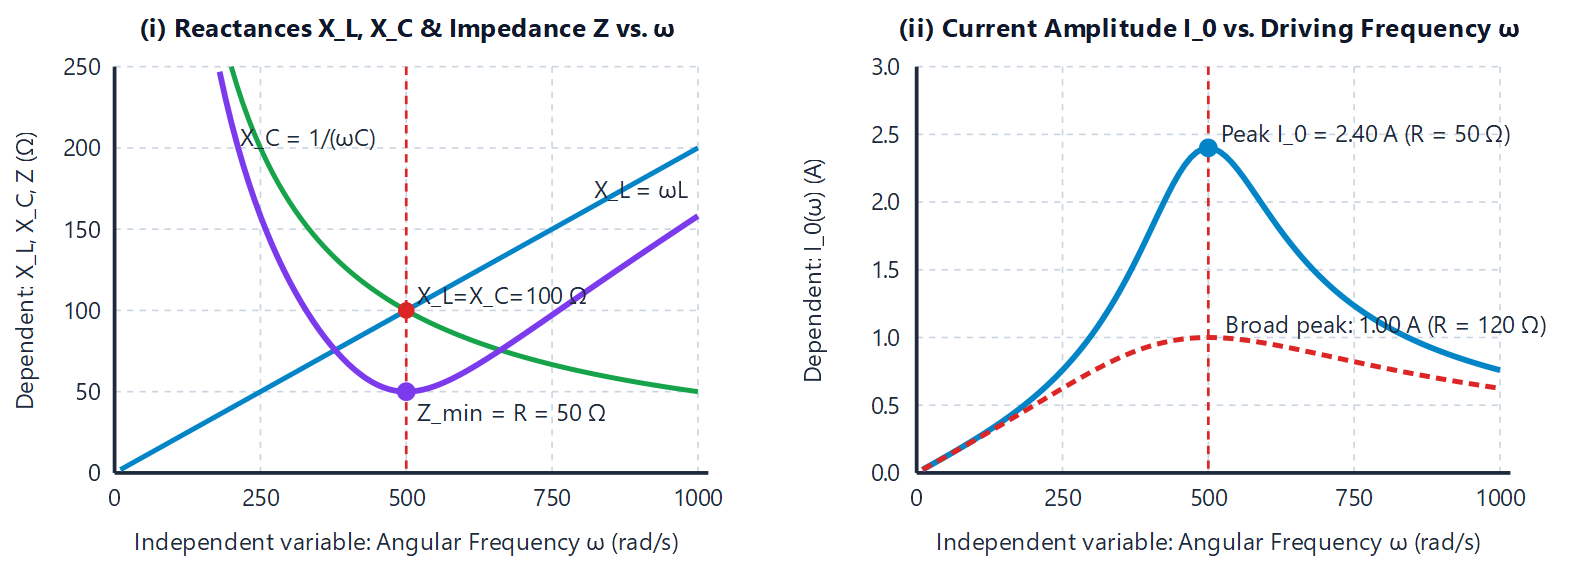
\includegraphics[width=0.82\linewidth]{day1_assets/s5-q4-grid-solved.png}\end{center}
\begin{center}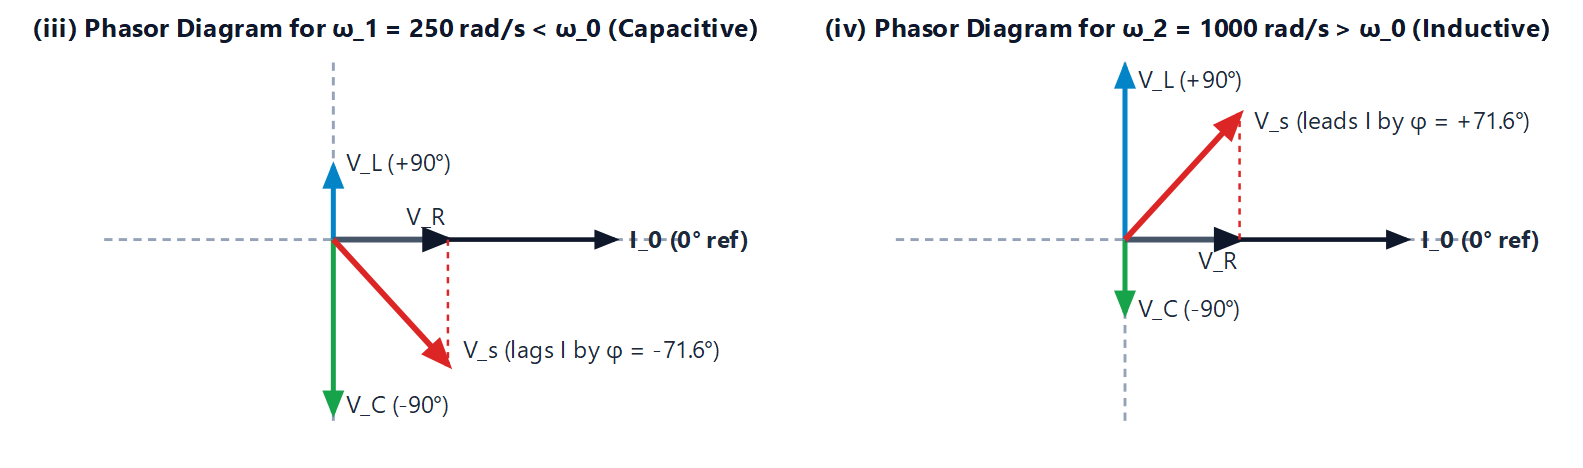
\includegraphics[width=0.82\linewidth]{day1_assets/s5-q4-phasors-solved.png}\end{center}

\end{document}
